\documentclass[24pt,ignorenonframetext,]{beamer}

\usepackage{pgfplots}
\usepackage{tikz}
\pgfdeclarelayer{edgelayer}
\pgfdeclarelayer{nodelayer}
\pgfsetlayers{edgelayer,nodelayer,main}
\tikzstyle{rect}=[rectangle,fill=white,draw=black]
%\tikzstyle{vol}=[rectangle,fill=DeepSkyBlue,draw=DeepSkyBlue]
%\tikzstyle{volb}=[rectangle,fill=Blue,draw=Blue]
%\tikzstyle{scircle}=[circle,fill=White,draw=Black]
%\tikzstyle{diamond}=[shape=diamond,fill=White,draw=Black]
\tikzstyle{simple}=[-,draw=black]
\tikzstyle{tick}=[-,draw=black,postaction={decorate},decoration={markings,mark=at position .5 with {\draw (0,-0.1) -- (0,0.1);}},line width=2.000]
\tikzstyle{darrow}=[latex-latex,draw=black]
\tikzstyle{arrow}=[-latex,draw=black]
\newcommand\drawline[1][black]{
    \begin{tikzpicture}
        \draw[#1, ultra thick] (0pt,3pt) -- (16pt,3pt);
        \draw[white] (0pt,0pt) -- (18pt,0pt);
    \end{tikzpicture}
}

% footer
\setbeamertemplate{footline}[text line]{%
  \parbox{0.333\linewidth}{
    \vspace*{-8pt}\centering \insertshortauthor
  }
  \hfill
  \parbox{0.333\linewidth}{
    \vspace*{-8pt}\raggedleft TUM MW BioVT
  }
  \hfill
  \parbox{0.333\linewidth}{
    \vspace*{-8pt}\raggedleft\insertpagenumber
  }
}

% captions
\setbeamertemplate{caption}[default]
\setbeamertemplate{caption label separator}{: }
\setbeamercolor{caption name}{fg=normal text.fg}

\beamertemplatenavigationsymbolsempty
\usepackage{lmodern}
\usepackage{amssymb,amsmath}
\usepackage{ifxetex,ifluatex}
\usepackage{fixltx2e} % provides \textsubscript
\ifnum 0\ifxetex 1\fi\ifluatex 1\fi=0 % if pdftex
  \usepackage[T1]{fontenc}
  \usepackage[utf8]{inputenc}
  \usepackage{eurosym}
\else % if luatex or xelatex
  \ifxetex
    \usepackage{mathspec}
  \else
    \usepackage{fontspec}
  \fi
  \defaultfontfeatures{Ligatures=TeX,Scale=MatchLowercase}
  \newcommand{\euro}{€}
    \setmainfont[]{Source Serif Pro}
    \setsansfont[]{Source Sans Pro}
    \setmonofont[Mapping=tex-ansi]{Source Code Pro}
\fi
\usecolortheme{biovt}
\usefonttheme{serif} % use mainfont rather than sansfont for slide text
% use upquote if available, for straight quotes in verbatim environments
\IfFileExists{upquote.sty}{\usepackage{upquote}}{}
% use microtype if available
\IfFileExists{microtype.sty}{%
\usepackage{microtype}
\UseMicrotypeSet[protrusion]{basicmath} % disable protrusion for tt fonts
}{}
\newif\ifbibliography

% Prevent slide breaks in the middle of a paragraph:
\widowpenalties 1 10000
\raggedbottom

\AtBeginPart{
  \let\insertpartnumber\relax
  \let\partname\relax
  \frame{\partpage}
}
\AtBeginSection{
  \ifbibliography
  \else
    \let\insertsectionnumber\relax
    \let\sectionname\relax
    \frame{\sectionpage}
  \fi
}
\AtBeginSubsection{
  \let\insertsubsectionnumber\relax
  \let\subsectionname\relax
  \frame{\subsectionpage}
}

\setlength{\parindent}{0pt}
\setlength{\parskip}{6pt plus 2pt minus 1pt}
\setlength{\emergencystretch}{3em}  % prevent overfull lines
\providecommand{\tightlist}{%
  \setlength{\itemsep}{0pt}\setlength{\parskip}{0pt}}
\setcounter{secnumdepth}{0}

\title{Development of a Low-Cost Electrical Conductivity Meter for Liquids}
\author{Sebastian Plamauer}
\date{22.08.2016}



\begin{document}
\frame{\titlepage}

\begin{frame}{Outline}

\begin{itemize}
\tightlist
\item
  Introduction
\item
  Objectives
\item
  Design
\item
  Results
\item
  Outlook
\end{itemize}

\end{frame}

\begin{frame}{Introduction}

\begin{figure}
    \begin{center}
    \begin{tikzpicture}[scale=0.7]
        \node[,inner sep=0] at (0,0) {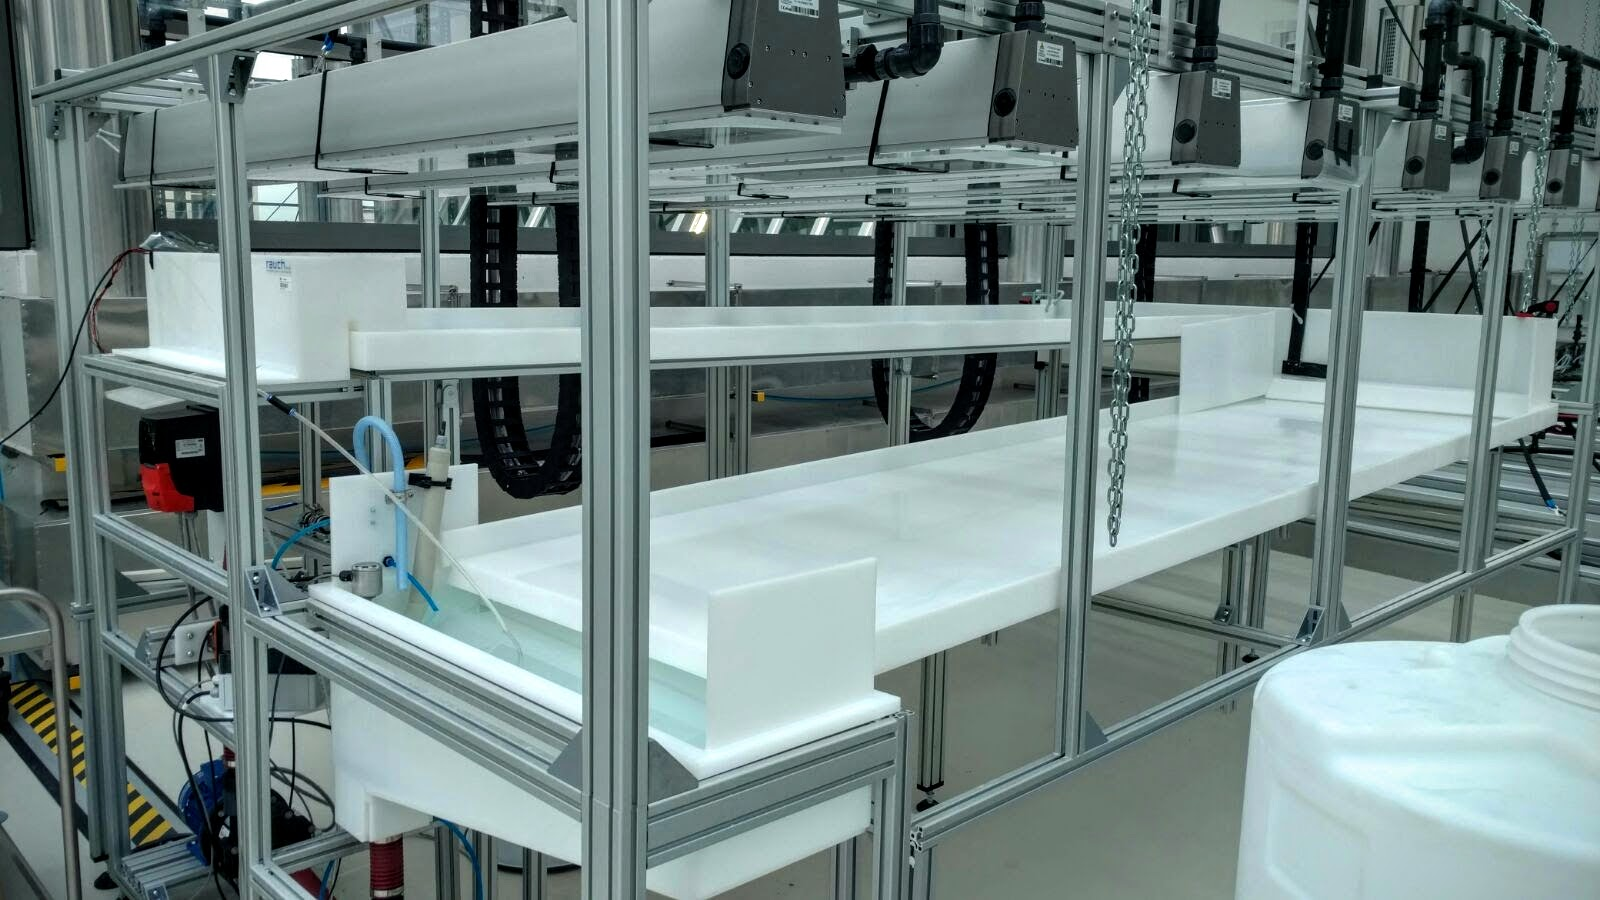
\includegraphics[width=\textwidth]{../thesis/images/pbr.jpg}};
        \draw[red!80!blue,ultra thick] (-5,1.5) ellipse (1.75 and 1.25);
        \draw[green!80!blue,ultra thick] (-2,-2) ellipse (3.25 and 2.25);
        \draw[-latex, blue!80!white, ultra thick] (-0.9,1.1) -- (2,1.15);
        \draw[-latex, blue!80!white, ultra thick] (2.25,-0.45) -- (0.85,-0.8);
        \draw[-latex, blue!80!white, ultra thick] (4.5,1) .. controls (5,0.75) and (4.5,0) ..  (3.75,-0.15);
    \end{tikzpicture}
        %\caption[The photobioreactor for which the conductivity meter is developed]{The photobioreactor for which the conductivity meter is developed - Water enters through the inlet basin, (\drawline[red!80!blue]), streams down the ramp (\drawline[blue!80!white,-latex]) to the collection tank (\drawline[green!80!blue]) from where it is pumped back to the inlet.}
        \label{fig:pbr}
    \end{center}
\end{figure}

\end{frame}

\begin{frame}{Objectives}

enable experiments to validate simulation

\begin{itemize}
\tightlist
\item
  add saltwater impulse to freshwater stream
\item
  measure changes in salinity over time

  \begin{itemize}
  \tightlist
  \item
    at multiple points
  \item
    fast
  \end{itemize}
\end{itemize}

\end{frame}

\begin{frame}

\begin{block}{Requirements}

\begin{itemize}
\tightlist
\item
  spacial resolution: 10mm
\item
  sensitivity: 0.1\%
\item
  range: 0 to 2.5\%
\item
  cost per sensor: \textless{} \euro{}25
\item
  deployable in the algae reactor
\item
  easy to use
\end{itemize}

\end{block}

\end{frame}

\begin{frame}{Design}

\begin{figure}
    \begin{center}
\begin{tikzpicture}[scale=0.65]
    \fill [fill=yellow, opacity=0.25] (-5.5,4) rectangle (5.2,7);
    \fill [fill=green, opacity=0.25] (-5.5,-3.5) rectangle (5.2,4);
    \fill [fill=blue, opacity=0.25] (5.2,-3.5) rectangle (10,2);
    \begin{pgfonlayer}{nodelayer}
        \node [rounded corners=8pt, inner sep=8pt, style=rect] (0) at (8, -1) {8 Electrodes};
        \node [rounded corners=8pt, inner sep=8pt, style=rect] (1) at (0, 3) {Microcontroller};
        \node [rounded corners=8pt, inner sep=8pt, style=rect] (2) at (-3, -1) {MinieC Interface};
        \node [rounded corners=8pt, inner sep=8pt, style=rect] (3) at (3, 0.25) {Matrix Switch};
        \node [rounded corners=8pt, inner sep=8pt, style=rect] (4) at (0, 6) {PC};
        \node [style=rect, inner sep=8pt, rounded corners=8pt] (5) at (3, -2.25) {Matrix Switch};
    \end{pgfonlayer}
    \begin{pgfonlayer}{edgelayer}
        \draw [style=darrow] (4) to node[left]{USB} (1);
        \draw [style=simple, bend right=15, looseness=1.00] (0) to node[above]{8 SIG} (3);
        \draw [style=simple, bend right=15, looseness=1.00] (3) to node[above]{SIG} (2);
        \draw [style=arrow, bend left=15, looseness=1.00] (1) to node[right]{SPI} (3);
        \draw [style=darrow, bend right=15, looseness=1.00] (1) to node[left]{I2C} (2);
        \draw [style=simple, bend right=15, looseness=1.00] (2) to node[below]{GND} (5);
        \draw [style=simple, bend right=15, looseness=1.00] (5) to node[below]{8 GND} (0);
        \draw [style=arrow, bend left=15, looseness=1.00] (1) to node[right, pos=0.9]{SPI} (5);
    \end{pgfonlayer}
        \draw (-5.5,-3.5) -- (10,-3.5) -- (10,2) node[below, left, yshift=-8pt] {$n$} -- (-5.5,2) -- (-5.5,-3.5);
\end{tikzpicture}
        %\begin{tikzpicture}
	\begin{pgfonlayer}{nodelayer}
		\node [rounded corners=8pt, inner sep=16pt, style=rect] (0) at (8, -1) {8 Electrodes};
		\node [rounded corners=8pt, inner sep=16pt, style=rect] (1) at (0, 3) {Microcontroller};
		\node [rounded corners=8pt, inner sep=16pt, style=rect] (2) at (-3, -1) {MinieC Interface};
		\node [rounded corners=8pt, inner sep=16pt, style=rect] (3) at (3, 0.25) {Matrix Switch};
		\node [rounded corners=8pt, inner sep=16pt, style=rect] (4) at (0, 6) {PC};
		\node [style=rect, inner sep=16pt, rounded corners=8pt] (5) at (3, -2.25) {Matrix Switch};
	\end{pgfonlayer}
	\begin{pgfonlayer}{edgelayer}
		\draw [style=darrow] (4) to node[left]{USB} (1);
		\draw [style=simple, bend right=15, looseness=1.00] (0) to node[above]{8 SIG} (3);
		\draw [style=simple, bend right=15, looseness=1.00] (3) to node[above]{SIG} (2);
		\draw [style=arrow, bend left=15, looseness=1.00] (1) to node[right]{SPI} (3);
		\draw [style=darrow, bend right=15, looseness=1.00] (1) to node[left]{I2C} (2);
		\draw [style=simple, bend right=15, looseness=1.00] (2) to node[below]{GND} (5);
		\draw [style=simple, bend right=15, looseness=1.00] (5) to node[below]{8 GND} (0);
		\draw [style=arrow, bend left=15, looseness=1.00] (1) to node[right, pos=0.9]{SPI} (5);
	\end{pgfonlayer}
\end{tikzpicture}
        %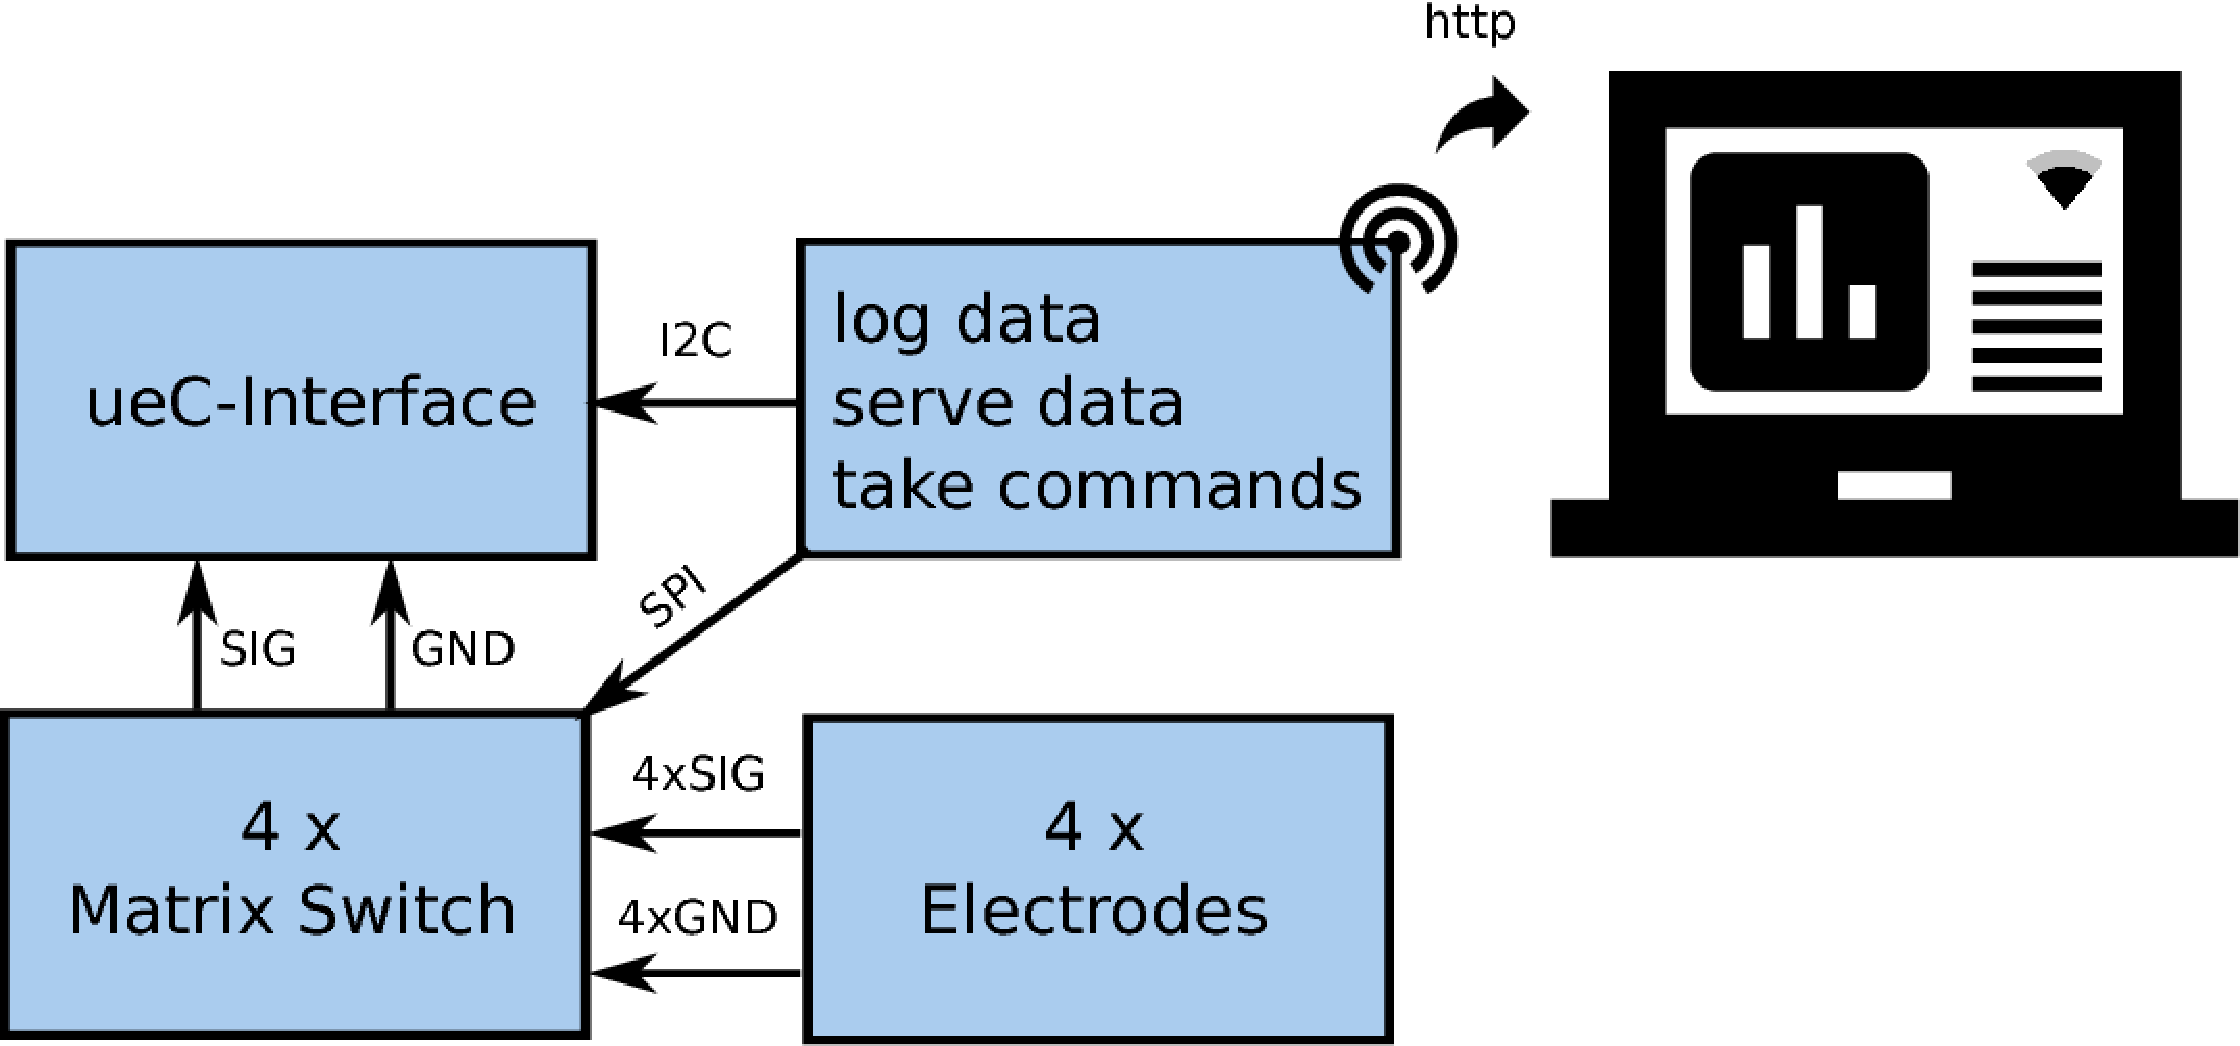
\includegraphics[width=\textwidth]{images/systemdesign.pdf} 
        %\caption[System Design]{System Design - The yellow area marks the user interface of the system, the green area is the hardware that is mounted on the carrier board and the blue area shows the sensors deployed in the water stream. The rectangle marks the parts of the system that is repeated $n$ times to get to the needed number of sensors.}
        \label{fig:sys}
    \end{center}
\end{figure}

\end{frame}

\begin{frame}

\begin{block}{finished Hardware}

\begin{figure}
    \begin{center}
        \begin{tikzpicture}[scale=0.7]
            \node[,inner sep=0] at (0,0) {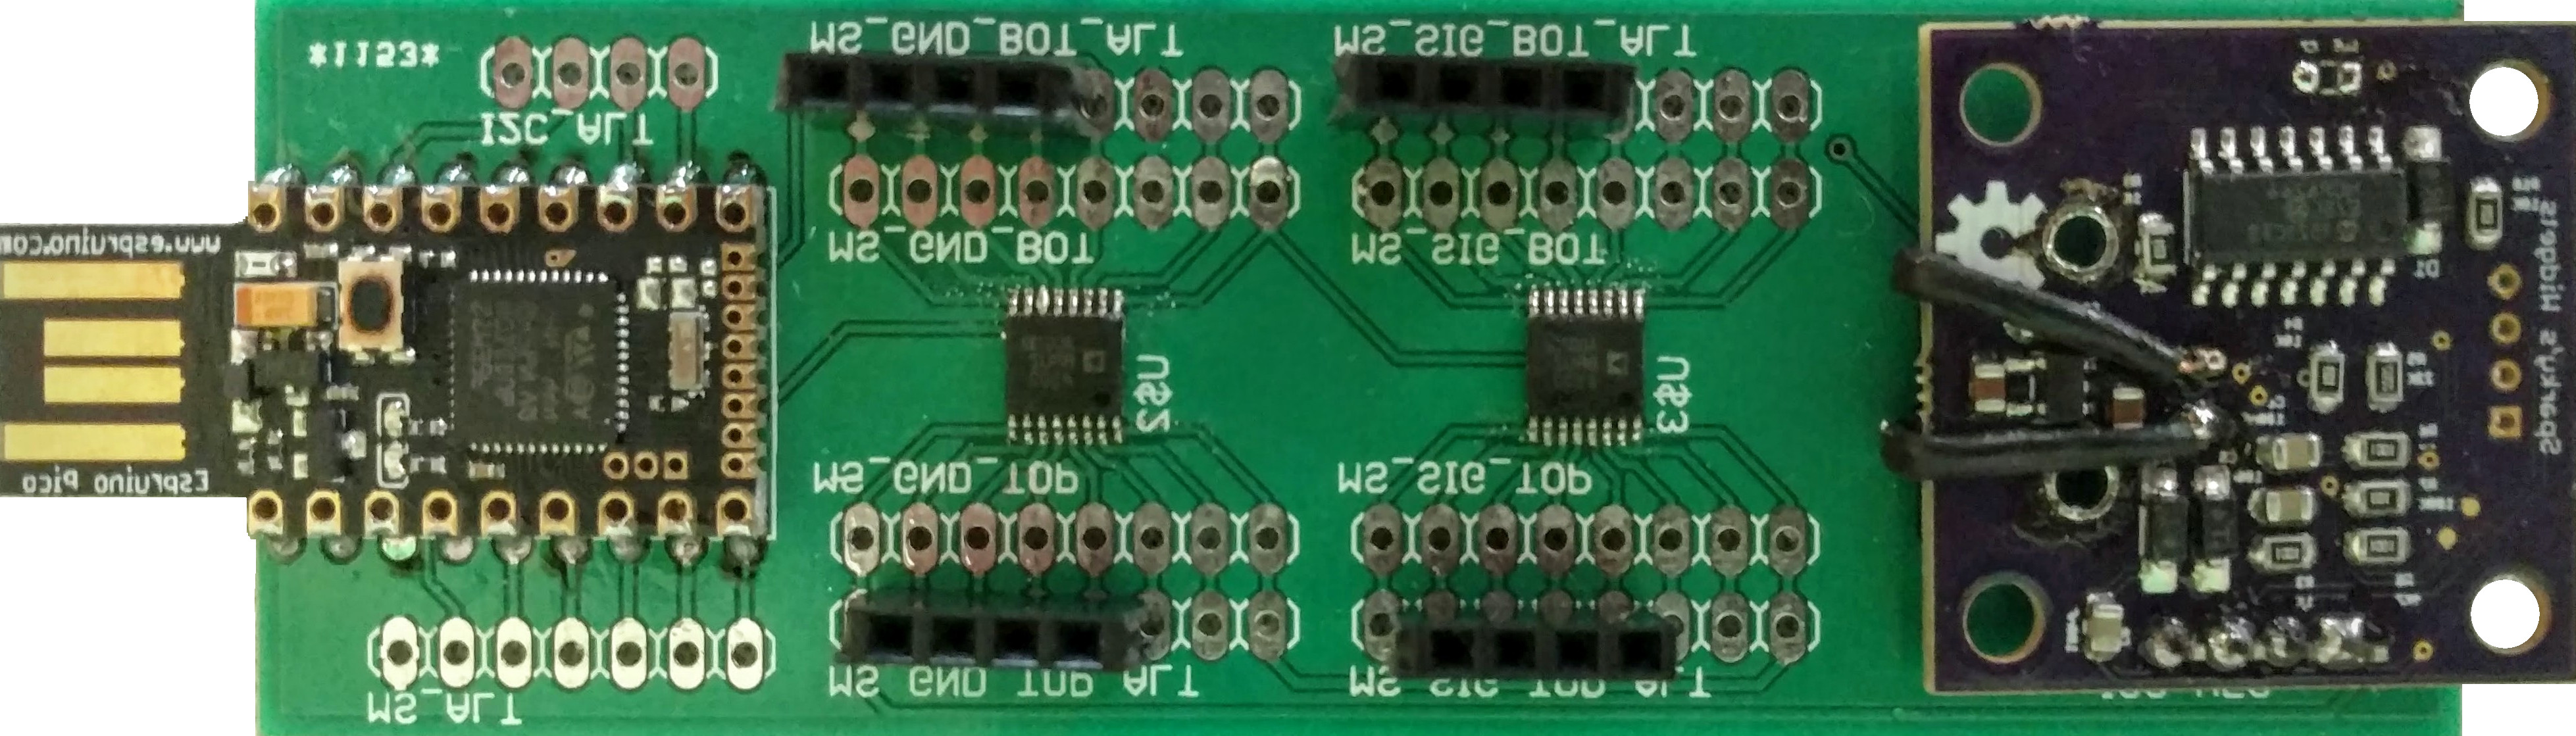
\includegraphics[width=0.5\textwidth]{../thesis/images/cb.jpg}};
            \node[inner sep=0] at (0,-3) {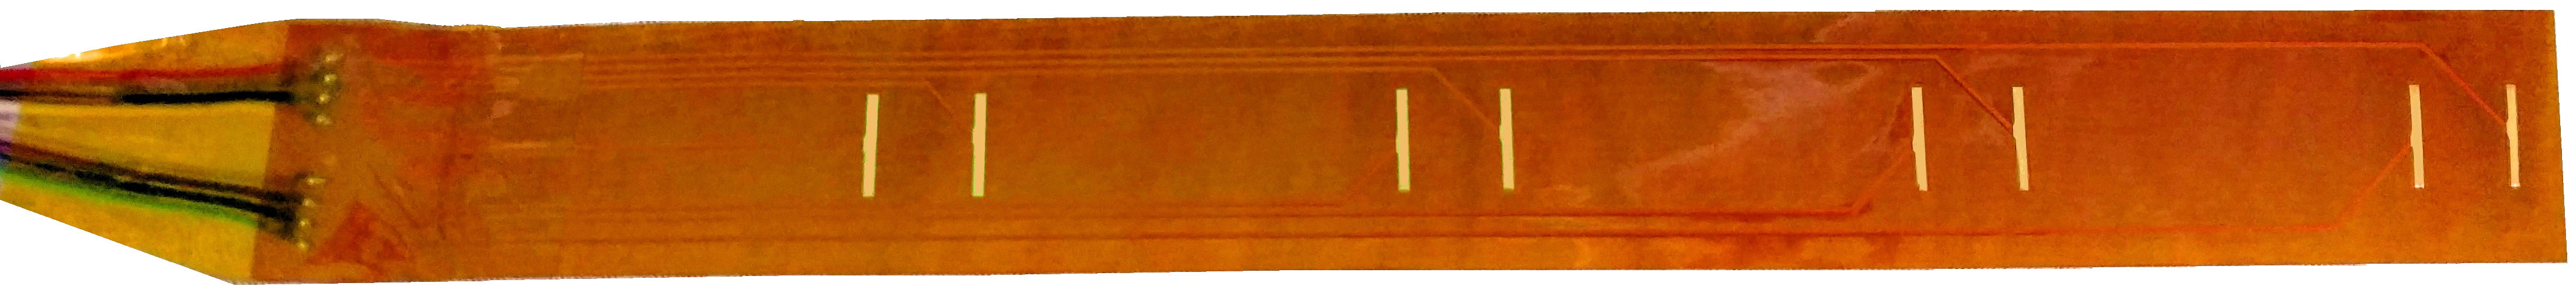
\includegraphics[width=\textwidth]{../thesis/images/fpcbp.jpg}};
            
            \draw[red,ultra thick,rounded corners] (-4,-0.75) rectangle (-1.5,0.75);
            
            \draw[red!40!yellow,ultra thick,rounded corners] (-1,-0.35) rectangle (-0.25,0.35);
            \draw[red!40!yellow,ultra thick,rounded corners] (0.55,-0.35) rectangle (1.3,0.35);
            
            \draw[red!25!yellow,ultra thick,rounded corners] (-1.45,-1) rectangle (-0.3,-0.6);
            \draw[red!25!yellow,ultra thick,rounded corners] (0.3,-1.05) rectangle (1.3,-0.65);
            \draw[red!25!yellow,ultra thick,rounded corners] (-1.54,1.05) rectangle (-0.44,0.65);
            \draw[red!25!yellow,ultra thick,rounded corners] (0.15,1.05) rectangle (1.15,0.65);
            
            \draw[blue,ultra thick,rounded corners] (1.8,-1.2) rectangle (4,1.2);
            \draw[green,ultra thick,rounded corners] (-8,-4) rectangle (8,-2);
            \draw[blue!50!white,ultra thick,rounded corners] (-2.75,-3.5) rectangle (-1.65,-2.5);
        \end{tikzpicture}
        %\caption[The developed sensor system]{The developed sensor system - The microcontroller and USB connection (\drawline[red,ultra thick]) control all parts and connect to the host PC. The matrix switches (\drawline[red!40!yellow,ultra thick]) connect the MinieC (\drawline[blue,ultra thick]) to the sensor strip (\drawline[green,ultra thick]) containing the sensors (\drawline[blue!50!white,ultra thick]) via the connectors (\drawline[red!25!yellow,ultra thick]).}
        \label{fig:isys}
    \end{center}
\end{figure}

\end{block}

\end{frame}

\begin{frame}{Results}

\end{frame}

\begin{frame}

\begin{block}{Demo}

\end{block}

\end{frame}

\begin{frame}{Outlook}

\begin{figure}
    \begin{center}
        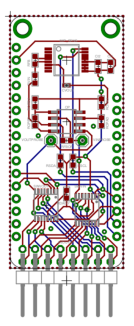
\includegraphics[height=225pt]{images/wing.pdf}
    \end{center}
\end{figure}

\end{frame}

\end{document}
